\documentclass[
  11pt,
  letterpaper,
   addpoints,
   %answers
  ]{exam}

\usepackage{../exercise-preamble}

\begin{document}

\noindent
\begin{minipage}{0.47\textwidth}

\includegraphics[width=\textwidth]{../fcfm_die}
\end{minipage}
\begin{minipage}{0.53\textwidth}
\begin{center} 
\large\textbf{Electromagnetismo Aplicado} (EL3103-1) \\
\large\textbf{Control 2} \\
\normalsize Prof.~Benjamin Jacard H.\\
\normalsize Prof.~Aux.~Erik Saez A.
\end{center}
\end{minipage}

\vspace{0.5cm}
\noindent
\vspace{.85cm}

\begin{questions}
    %%%%%%%%%%%%%%%%%%%%%%%%%%%%
    \question     
    Considere una onda plana cuyo campo eléctrico está dado por:$ \vec{E} = E_0 e^{-jk_0 z} e^{j\omega t} \hat{i}$
incide normalmente desde el aire en la interfaz plana de una placa dieléctrica (\( \varepsilon = \varepsilon_r \varepsilon_0 \)) de espesor \( d \), adosada a una placa perfectamente conductora.

\vspace{0.5em}

\begin{enumerate}
    \item[i)] Plantee las expresiones de los campos \( \vec{E} \) y \( \vec{H} \) (vectores-fasores) en el aire y en el dieléctrico en función de los datos, considerando propagación según \( z^+ \) y \( z^- \).(\textbf{2 Pts})
    
    \item[ii)] Deduzca la expresión del coeficiente de reflexión complejo \( \Gamma \) en la interfaz \( z = -d \). (\textbf{2 Pts})
    \[
    \Gamma = \frac{E_{1}^{-} e^{-kk_{o}d}}{E_{0}e^{jk_{o}d}} 
    \]
    
    \item[iii)] Determine y compare la potencia que transmite la onda incidente y la onda reflejada en el medio 1, considerando una unidad de área en el plano \( xy \). (\textbf{2 Pts})
\end{enumerate}
    
\begin{center}
    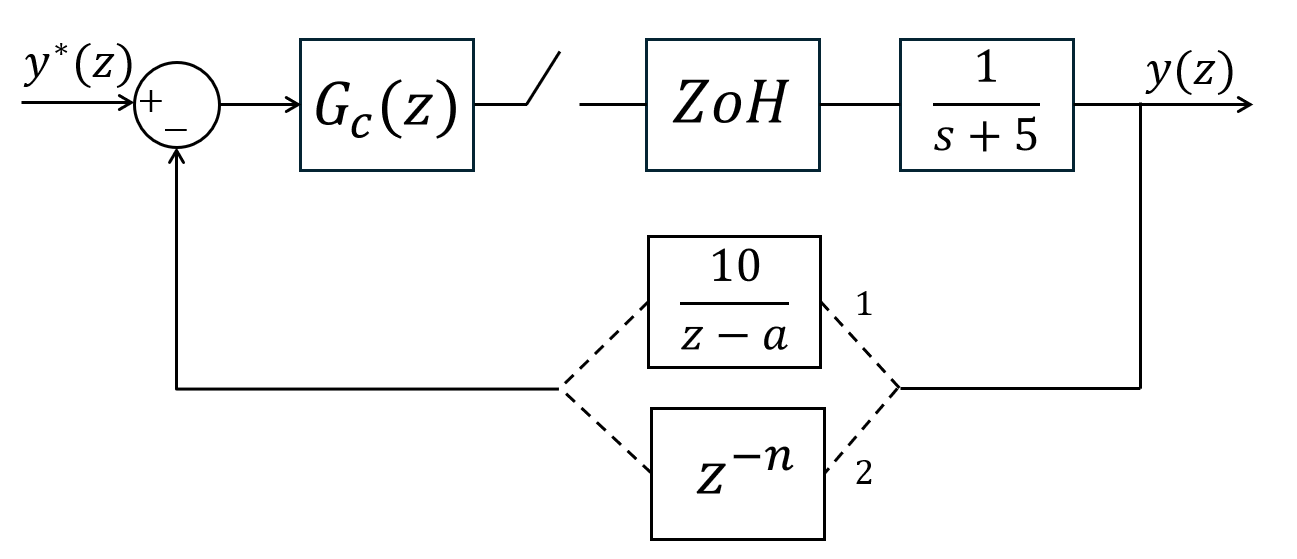
\includegraphics[width=0.45\textwidth]{Control_2_1}
    \captionof{figure}{Esquema del problema}
\end{center}
    %%%%%%%%%%%%%%%%%%%%%%%%%%%%
    \begin{solution}
   
    \end{solution}
    %%%%%%%%%%%%%%%%%%%%%%%%%%%
    \newpage
    \question   En el dispositivo de la figura, base de funcionamiento de un amperímetro de tenaza, se desea determinar la relación entre el valor de la corriente que lleva el alambre recto y el voltaje que se mide en el voltímetro \(V\), conectado a un enrrollado de \(N\) vueltas muy juntas en el toroide de la figura.
    

    \begin{enumerate}
        \item[a)] El campo \(H\) y el campo \(E\) en el núcleo magnético y en el entrehierro del toroide. (\textbf{3 Pts})
        \item[b)] El valor instantáneo y el valor efectivo del voltaje inducido en los terminales del arrollado, y su relación con \(I_0\). (\textbf{3 Pts})
    \end{enumerate}
    
    \textbf{Nota:}
    \begin{itemize}
        \item Suponga que en la sección transversal del núcleo y del entrehierro, el campo \(H\) es uniforme e igual al existente en el centro de la sección transversal \((R=(a+b)/2)\).
        \item En el alambre recto, la expresión fasorial de la corriente que se quiere medir es \(I_0 e^{j\omega t}\).
        \item Desprecie efectos de borde en el entrehierro.
        \item Suponga que el voltímetro es ideal, de modo que su impedancia equivalente es infinita.
        \item Como el toroide es delgado, una buena aproximación es utilizar coordenadas cilíndricas para determinar volúmenes e interfaces del núcleo magnético y del entrehierro de abertura \(g\).
    \end{itemize}
    \begin{center}
        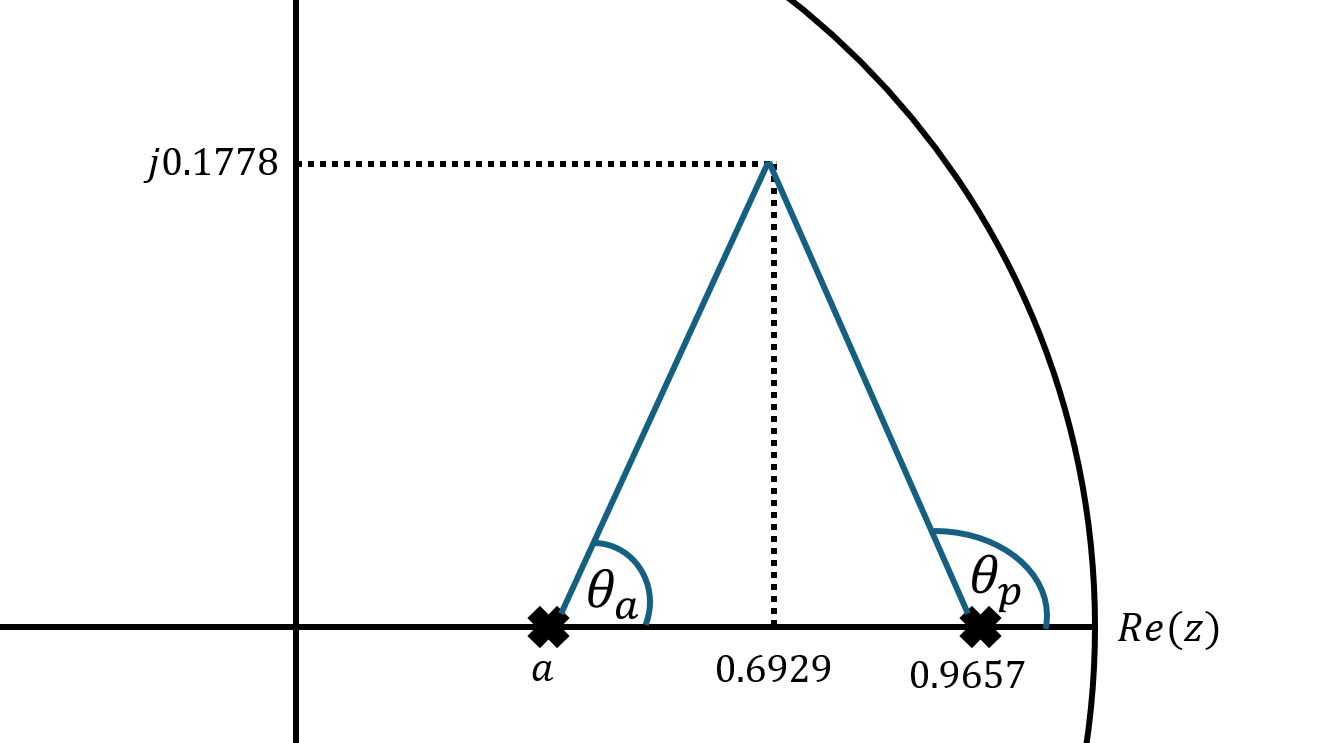
\includegraphics[width=0.5\textwidth]{Control_2_2}
        \captionof{figure}{Esquema del problema}
    \end{center}
    %%%%%%%%%%%%%%%%%%%%%%%%%%%
    \begin{solution}
       a
\end{solution}
%%%%%%%%%%%%%%%%%%%%%%%%%%%

\end{questions}
%%%%%%%%%%%%%%%%%%%%%%%%%%%

\end{document}